\section{Folgerungen und Anwendungen der Compton-Formel}

Die Compton-Formel lautet:
\[
\Delta \lambda = \lambda' - \lambda = \frac{h}{m_e c}(1 - \cos\theta)
\]

\begin{PhysikBox}[Physikalische Bedeutung]
	Die Compton-Formel beschreibt die Zunahme der Wellenlänge \(\Delta \lambda\)
	eines Photons nach elastischer Streuung an einem Elektron. 
	Die Verschiebung hängt nur vom Streuwinkel \(\theta\) ab – 
	nicht von der Energie des einfallenden Photons.
\end{PhysikBox}



\subsection*{Maximale Compton-Verschiebung}

Der maximale Wert ergibt sich für \( \theta = 180^\circ \), da hier \( 1 - \cos(180^\circ) = 2 \). Damit:

\begin{align*}
	\Delta \lambda_\text{max} &= 2 \cdot \frac{h}{m_e c}
	= 2 \cdot \frac{6{,}626 \cdot 10^{-34}~\text{Js}}{9{,}109 \cdot 10^{-31}~\text{kg} \cdot 3{,}0 \cdot 10^8~\text{m/s}}\\
	&= 4{,}85 \cdot 10^{-12}~\text{m}
\end{align*}



\begin{DidaktikBox}[Der Compton-Wellenlängenfaktor]
	Die Größe
	\[
	\lambda_C = \frac{h}{m_e c} = 2{,}43 \times 10^{-12}~\text{m}
	\]
	heißt \emph{Compton-Wellenlänge des Elektrons}.  
	Sie ist eine fundamentale Naturkonstante, die angibt, 
	wie stark Photonen bei maximaler Rückstreuung (\(\theta=180^\circ\)) 
	ihre Wellenlänge ändern.
\end{DidaktikBox}


\subsection*{Vergleich für verschiedene Strahlungsarten}

Diese Wellenlängenverschiebung ist nun im Vergleich zu typischen Photonen-Wellenlängen zu betrachten:

\begin{center}
	\begin{tabular}{|l|c|c|c|}
		\hline
		\textbf{Strahlungsart} & \(\lambda\) [m] & \(\Delta \lambda\) [m] & \(\frac{\Delta \lambda}{\lambda}\) \\
		\hline
		Rotes Licht & \(7{,}0 \cdot 10^{-7}\) & \(4{,}85 \cdot 10^{-12}\) & \(6{,}93 \cdot 10^{-6}\) \\
		Röntgenstrahlung & \(1{,}0 \cdot 10^{-11}\) & \(4{,}85 \cdot 10^{-12}\) & \(0{,}485\) \\
		Gammastrahlung & \(1{,}0 \cdot 10^{-13}\) & \(4{,}85 \cdot 10^{-12}\) & \(48{,}5\) \\
		\hline
	\end{tabular}
\end{center}

\begin{HinweisBox}[Vergleich mit dem sichtbaren Bereich]
	Für sichtbares Licht (\(\lambda \approx 700\,\text{nm}\)) ist die relative Änderung \(\Delta \lambda / \lambda \) 
	verschwindend klein, während sie für Röntgen- und Gammastrahlung deutlich messbar ist.
\end{HinweisBox}



\subsection*{Fazit}

\begin{itemize}
	\item Bei sichtbarem Licht (z.\,B. \( \lambda = 700\,\text{nm} \)) ist die Compton-Verschiebung praktisch unmessbar.
	\item Im Röntgenbereich ist \(\Delta \lambda\) vergleichbar mit \(\lambda\); der Effekt ist experimentell gut nachweisbar.
	\item Für Gammastrahlung übersteigt \(\Delta \lambda\) die ursprüngliche Wellenlänge deutlich.
\end{itemize}

\begin{PhysikBox}[Warum Röntgenstrahlen?]
	Der Compton-Effekt wurde 1923 mit Röntgenstrahlung entdeckt, 
	weil nur in diesem Energiebereich die Wellenlängenverschiebung messbar groß ist.  
	Bei sichtbarem Licht wäre der Effekt um viele Größenordnungen zu klein.
\end{PhysikBox}

\newpage
\noindent

\subsection*{Relative Compton-Verschiebung in Abhängigkeit von der Wellenlänge}

\begin{figure}[h]
	\centering
	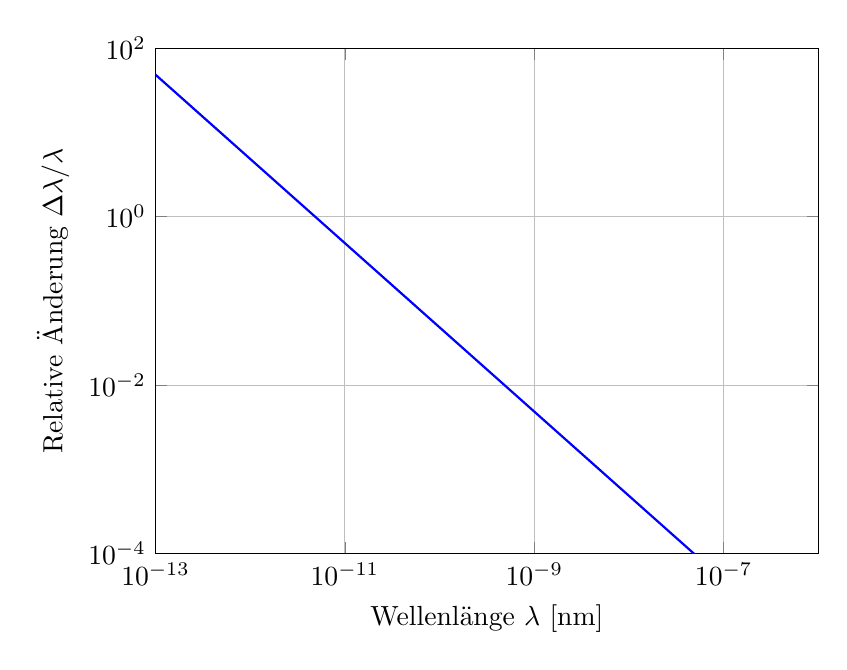
\begin{tikzpicture}
		\begin{axis}[
			width=10cm,
			height=8cm,
			xlabel={Wellenlänge $\lambda$ [nm]},
			ylabel={Relative Änderung $\Delta \lambda / \lambda$},
			xmode=log,
			ymode=log,
			grid=both,
			minor grid style={gray!20},
			major grid style={gray!50},
			domain=1e-13:1e-6,
			samples=500,
			xmin=1e-13, xmax=1e-6,
			ymin=1e-4, ymax=1e2,
			xtick={1e-13,1e-11,1e-9,1e-7},
			xticklabels={$10^{-13}$, $10^{-11}$, $10^{-9}$, $10^{-7}$},
			ytickten={-4,-2,0,2}
			]
			\addplot [
			thick,
			blue
			]
			expression {
				4.849416e-12 / x
			};
		\end{axis}
	\end{tikzpicture}
	\caption{Relative Wellenlängenänderung $\Delta \lambda / \lambda$ gemäß der Compton-Formel für $\theta = 180^\circ$ in Abhängigkeit von der einfallenden Wellenlänge $\lambda$.}
\end{figure}
